\documentclass[11pt,a4paper]{article}

\usepackage[margin=1in]{geometry}
\usepackage[T1]{fontenc}
\usepackage{lmodern}
\usepackage{microtype}
\usepackage{setspace}
\usepackage{longtable}
\usepackage{array}
\usepackage{booktabs}
\usepackage{tabularx}
\usepackage{enumitem}
\usepackage{xcolor}
\usepackage{hyperref}
\usepackage{tikz}
\usetikzlibrary{shapes.geometric,arrows.meta,positioning,fit,backgrounds,calc,shapes.symbols}

\hypersetup{
    colorlinks=true,
    linkcolor=blue!60!black,
    urlcolor=blue!60!black,
}

\onehalfspacing
\setlength{\parskip}{0.5em}
\setlength{\parindent}{0pt}

\renewcommand{\arraystretch}{1.25}
\newcolumntype{L}[1]{>{\raggedright\arraybackslash}p{#1}}

% TikZ styles for DFDs and use case diagrams
\tikzset{
    process/.style={circle, draw, thick, minimum size=2.2cm, align=center, font=\small},
    extproc/.style={rectangle, draw, thick, minimum width=2.6cm, minimum height=1.0cm, align=center, font=\small},
    datastore/.style={rectangle, draw, thick, minimum width=3.0cm, minimum height=0.9cm, align=center, font=\small\itshape},
    flow/.style={-{Stealth[length=2.5mm]}, thick},
    actor/.style={font=\small, align=center},
    usecase/.style={ellipse, draw, thick, minimum width=3.2cm, minimum height=1.0cm, align=center, font=\small},
    boundary/.style={rectangle, draw, thick, rounded corners=2pt, inner sep=10pt},
}

\title{\textbf{Software Requirements Specification} \\[0.4em] \large SwishVision: Basketball Analytics Platform}
\author{Mallick Mikaal Imam \and Minhaj ul Hassan \and Muhammad Ahmed Silat \and Syed Muhammad Sameer Hassan}
\date{Version 1.10 \\ 11th May 2026}

\begin{document}

\maketitle
\thispagestyle{empty}

\begin{center}
\begin{tabular}{|L{6cm}|L{6cm}|}
\hline
\textbf{Project Team} & \\ \hline
Mallick Mikaal Imam & \\ \hline
Minhaj ul Hassan & \\ \hline
Muhammad Ahmed Silat & \\ \hline
Syed Muhammad Sameer Hassan & \\ \hline
\end{tabular}

\vspace{0.5em}
\begin{tabular}{|L{6cm}|L{6cm}|}
\hline
\textbf{Submission Date} & 11th May 2026 \\ \hline
\end{tabular}
\end{center}

\newpage

\section*{Document History}
\begin{longtable}{|c|L{3.5cm}|L{2.8cm}|L{6.5cm}|}
\hline
\textbf{Version} & \textbf{Name} & \textbf{Date} & \textbf{Description of Change} \\ \hline
1.00 & Ahmed Silat & 16 Mar 2026 & Initial draft, project proposal translated to SRS \\ \hline
1.10 & Minhaj ul Hassan & 11 May 2026 & Post-implementation update, locked in tech stack (FastAPI / React / SQL Server / Celery+Redis / JWT), reflected delivered scope, marked all use cases as implemented \\ \hline
1.11 & Minhaj ul Hassan & 11 May 2026 & Corrected output codec to H.264 MP4 (transcoded via \texttt{imageio-ffmpeg}); added \texttt{imageio-ffmpeg}, \texttt{supervision}, and \texttt{pandas} to the Software Interfaces inventory \\ \hline
\end{longtable}

\section*{Distribution List}
\begin{tabular}{|L{6cm}|L{6cm}|}
\hline
\textbf{Name} & \textbf{Role} \\ \hline
& Supervisor / Course Instructor \\ \hline
& Project Manager \\ \hline
\end{tabular}

\section*{Document Sign-Off}
\begin{tabular}{|c|L{4cm}|L{3cm}|L{3cm}|}
\hline
\textbf{Version} & \textbf{Sign-off Authority} & \textbf{Project Role} & \textbf{Sign-off Date} \\ \hline
1.00 & & Supervisor & \\ \hline
\end{tabular}

\newpage
\tableofcontents
\newpage

\section{Introduction}

\subsection{Purpose of Document}
The purpose of this document is to outline the requirements for the construction of SwishVision, a web-based basketball analytics platform. It documents functional and non-functional requirements, system constraints, interface requirements, design constraints, and other factors vital to ensuring the software meets its intended goals. It serves as the primary reference for development, validation, and stakeholder alignment.

\subsection{Intended Audience}
The intended audience includes the course supervisor, the project development team, and any future maintainers of the system. The development team requires this document to ensure that implementation efforts are aligned with the stated purpose of the software. Supervisors and evaluators use it to assess the completeness and clarity of requirements. Future developers or contributors may reference it to understand system boundaries and expected behaviors.

\subsection{Document Convention}
\begin{itemize}[leftmargin=*]
    \item Font: Arial (Latin Modern as LaTeX substitute)
    \item Size: 11
    \item Line Spacing: 1.5
\end{itemize}

\section{Overall System Description}

\subsection{Project Background}
Basketball players at the amateur and semi-professional level lack access to the kind of analytical feedback that professional athletes receive from coaching staff and sports scientists. Critical aspects of shooting mechanics, such as release angle, elbow alignment, and follow-through consistency, occur too rapidly to be reliably analyzed by the naked eye. Furthermore, there exist no affordable, accessible tools that can automatically process practice footage and return structured, data-driven feedback.

SwishVision addresses this gap by building a web-based platform that accepts uploaded basketball footage and returns detailed performance analytics powered by computer vision and pose estimation. A fully working command-line prototype already exists (\texttt{main.py}), capable of detecting ball trajectory, rim interaction, and player skeletal keypoints using YOLOv8-based models. The object detection model (\texttt{best.pt}) was fine-tuned over 13 training iterations on the Basketball-1 dataset sourced from Roboflow (Eagle Eye workspace, CC BY 4.0), which provides labeled bounding boxes for three classes: basketball, rim, and sports ball. Human pose estimation uses the pre-trained \texttt{yolov8m-pose.pt} model, tracking 17 body joint keypoints per player.

\subsection{Project Scope}
\begin{itemize}[leftmargin=*]
    \item Allow users to create accounts and upload basketball practice footage via a web interface.
    \item Process uploaded video using the existing CV pipeline: ball tracking, rim tracking, and human pose estimation.
    \item Detect shot attempts and classify them as made or missed based on ball-rim interaction.
    \item Analyze shooting form using skeletal keypoints and compute joint angles across frames.
    \item Generate a per-session report including shot percentage, consistency scores, and mechanical feedback.
    \item Display session history and allow longitudinal comparison of performance across sessions.
    \item Provide a personal analytics dashboard summarizing trends over time.
\end{itemize}

\subsection{Not In Scope}
\begin{itemize}[leftmargin=*]
    \item Real-time (live) video analysis, the system processes pre-recorded footage only.
    \item Multi-player team analytics, the current scope focuses on individual player analysis.
    \item Mobile native applications (iOS/Android), the platform is web-only.
    \item Analysis of non-shooting basketball actions such as dribbling, defense, or passing.
\end{itemize}

\subsection{Project Objectives}
The primary objective of SwishVision is to make professional-grade shooting analytics widely accessible for amateur basketball players. Specific objectives include:
\begin{itemize}[leftmargin=*]
    \item Automate the detection and classification of shot attempts with high accuracy.
    \item Provide quantifiable metrics for shooting form that are consistent and reproducible.
    \item Enable players to track their progress over time through a persistent session history.
    \item Present results in a format that is intuitive and actionable for non-technical users.
    \item Expose the underlying CLI pipeline through a web interface without requiring users to have any technical knowledge.
\end{itemize}

\subsection{Stakeholders}
\textbf{Amateur Basketball Players (End Users).} The primary users of the system. They upload footage, view their analytics, and act on the feedback provided. Their goal is to improve shooting form and track progress.

\textbf{Development Team.} Responsible for building the system. Must ensure the web platform correctly integrates with the existing CV pipeline and delivers results reliably.

\textbf{Course Supervisor.} Evaluates the project from an academic standpoint. Requires documentation, working demonstrations, and compliance with software engineering standards.

\subsection{Operating Environment}
\begin{itemize}[leftmargin=*]
    \item \textbf{Server:} Linux or Windows environment running Python 3.8+, supporting PyTorch and YOLOv8 inference.
    \item \textbf{Client:} Any modern web browser (Chrome, Firefox, Safari, Edge), no installation required.
    \item \textbf{GPU:} CUDA-compatible NVIDIA GPU strongly recommended on the server side (PyTorch 2.0+); CPU fallback supported but slower.
    \item \textbf{RAM:} Minimum 4\,GB; 8\,GB+ recommended.
    \item \textbf{Storage:} Minimum 10\,GB for model files, uploaded videos, and generated outputs.
    \item \textbf{Network:} Standard HTTPS internet connection for the client.
    \item \textbf{Output Codec:} H.264 in MP4 container, frames are written with OpenCV's \texttt{mp4v} fourcc and then transcoded to H.264 (\texttt{yuv420p}, \texttt{+faststart}) via \texttt{imageio-ffmpeg} so the result plays directly in \texttt{<video>} elements in all major browsers. If \texttt{imageio-ffmpeg} is unavailable the pipeline keeps the \texttt{mp4v} output as a fallback.
\end{itemize}

\subsection{System Constraints}
\begin{itemize}[leftmargin=*]
    \item Video processing is computationally intensive; processing time scales with video length and resolution.
    \item Accuracy of shot detection and pose estimation is constrained by video quality, camera angle, and lighting.
    \item The system relies on pre-trained YOLOv8 models (\texttt{best.pt} for ball/rim, \texttt{yolov8m-pose.pt} for human pose).
    \item The web application must handle asynchronous video processing, the upload and the results must be decoupled with a job queue or background worker.
\end{itemize}

\subsection{Assumptions \& Dependencies}
\begin{itemize}[leftmargin=*]
    \item Uploaded videos are recorded from a side-on or slightly elevated angle capturing both player and basket.
    \item The player being analyzed occupies the majority of the frame.
    \item The server environment has Python 3.8+, PyTorch 2.0+, Ultralytics YOLOv8, OpenCV, NumPy, and Matplotlib installed.
    \item Model files (\texttt{models/best.pt} and \texttt{models/yolov8m-pose.pt}) are present on the server.
    \item Users have a device capable of recording and uploading video.
    \item The existing CLI pipeline is treated as a stable subsystem, wrapped, not rewritten, by the web layer.
    \item Intermediate data files (\texttt{angs.txt}, \texttt{xy\_coords.txt}, \texttt{detections.txt}, \texttt{ball\_locl.txt}) are transient.
    \item Text reports are generated per video and stored in \texttt{reports/}.
\end{itemize}

\section{Software Development Methodology}
An \textbf{Incremental Development} methodology will be used. This choice is appropriate because:
\begin{itemize}[leftmargin=*]
    \item A functioning core (the CV pipeline) already exists and can serve as the first increment.
    \item Requirements for the web layer can be developed and validated progressively.
    \item Early increments can be demonstrated to the supervisor for feedback before more advanced features are built.
    \item The team can parallelize work on the backend processing pipeline and the frontend interface.
\end{itemize}

\textbf{Delivered Increments (all completed as of 11 May 2026):}

\begin{tabular}{|c|L{8cm}|L{3cm}|}
\hline
\textbf{Increment} & \textbf{Deliverable} & \textbf{Status} \\ \hline
1 & User registration/login + video upload endpoint & Delivered \\ \hline
2 & Background processing integration, pipeline runs on uploaded video via Celery & Delivered \\ \hline
3 & Shot detection results displayed on frontend (React) & Delivered \\ \hline
4 & Pose/form analysis results and report generation & Delivered \\ \hline
5 & Session history and longitudinal dashboard & Delivered \\ \hline
\end{tabular}

\section{System Analysis \& Requirement Gathering}
Requirements were gathered through the following approaches:
\begin{itemize}[leftmargin=*]
    \item \textbf{Prototype Analysis:} The existing CLI pipeline (\texttt{main.py}) was examined to understand its outputs, ball tracks, rim tracks, human keypoints, joint angles, ball-hand contact frames, shot start events, and output video.
    \item \textbf{README Review:} The project README was reviewed to extract the module inventory, model files, dataset information, and the pipeline's 12-step processing flow.
    \item \textbf{Output Inspection:} Sample reports and annotated videos in \texttt{output\_videos/} were reviewed.
    \item \textbf{Stub File Analysis:} \texttt{stubs\_utils.py} and intermediate files indicate the pipeline supports caching, which is reused in the web architecture.
    \item \textbf{Project Proposal Review:} The proposal was analyzed to extract goals, features, and value propositions.
    \item \textbf{Gap Analysis:} Differences between CLI outputs and web user needs drove web-specific requirements (auth, upload, async processing, results, dashboard).
\end{itemize}

\section{External Interface Requirements}

\subsection{Hardware Interfaces}
\begin{itemize}[leftmargin=*]
    \item Server machine with sufficient CPU/RAM for Python inference. CUDA-compatible NVIDIA GPU strongly recommended.
    \item End users require only a standard computer or smartphone with internet access and a web browser.
    \item A camera or smartphone capable of recording at minimum 720p resolution is recommended.
\end{itemize}

\subsection{Software Interfaces}
\begin{itemize}[leftmargin=*]
    \item \textbf{Python 3.8+}: core runtime for the CV pipeline.
    \item \textbf{Ultralytics YOLOv8} (\texttt{ultralytics>=8.0.0}).
    \item \textbf{PyTorch 2.0+} (\texttt{torch>=2.0.0}, \texttt{torchvision>=0.15.0}).
    \item \textbf{OpenCV} (\texttt{opencv-python>=4.8.0}), video reading, frame processing, initial frame writing (\texttt{mp4v} fourcc).
    \item \textbf{imageio-ffmpeg}: bundles a static \texttt{ffmpeg} binary used to transcode to browser-playable H.264 MP4.
    \item \textbf{supervision} + \textbf{pandas}: used by the trackers.
    \item \textbf{NumPy} (\texttt{numpy>=1.24.0}).
    \item \textbf{Matplotlib} (\texttt{matplotlib>=3.7.0}).
    \item \textbf{FastAPI} (\texttt{fastapi==0.135.3}, \texttt{uvicorn==0.42.0}).
    \item \textbf{React} (Create React App, Node.js 18+).
    \item \textbf{SQLAlchemy} 2.0 + \textbf{Alembic} 1.14.
    \item \textbf{Microsoft SQL Server 2019+} with \textbf{pyodbc} 5.3 (ODBC Driver 17).
    \item \textbf{Celery} 5.6 + \textbf{Redis} 7+.
    \item \textbf{JWT} (\texttt{python-jose}, \texttt{passlib[bcrypt]}, \texttt{bcrypt}).
    \item \textbf{Web Browser}: Chrome, Firefox, Safari, or Edge.
\end{itemize}

\subsection{Communications Interfaces}
\begin{itemize}[leftmargin=*]
    \item \textbf{HTTPS}: all client-server communication encrypted via TLS.
    \item \textbf{REST API}: frontend communicates with backend via HTTP/REST for upload, status polling, and results.
    \item \textbf{WebSocket or Polling}: for job status updates.
\end{itemize}

\section{Functional Requirements}

\subsection{Data Flow Diagrams}

\subsubsection*{Context Level DFD}
The user submits a video and receives back analytics. The platform internally invokes the CV Engine and interacts with the database.

\begin{center}
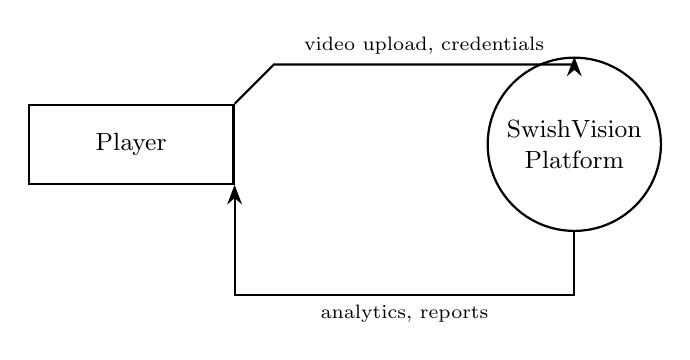
\begin{tikzpicture}[node distance=2.4cm and 3.2cm]
    \node[extproc] (user) {Player};
    \node[process, right=of user] (sys) {SwishVision\\Platform};

    \draw[flow] (user.north east) -- ++(0.5,0.5) -| node[above, pos=0.25, font=\scriptsize] {video upload, credentials} (sys.north);
    \draw[flow] (sys.south) |- ++(0,-0.8) -| node[below, pos=0.25, font=\scriptsize] {analytics, reports} (user.south east);
\end{tikzpicture}

\textit{Figure 1: Context Level DFD}
\end{center}

\subsubsection*{Level 0 DFD}
The system decomposes into five major processes: Authentication, Video Upload, CV Processing, Report Generation, and Dashboard.

\begin{center}
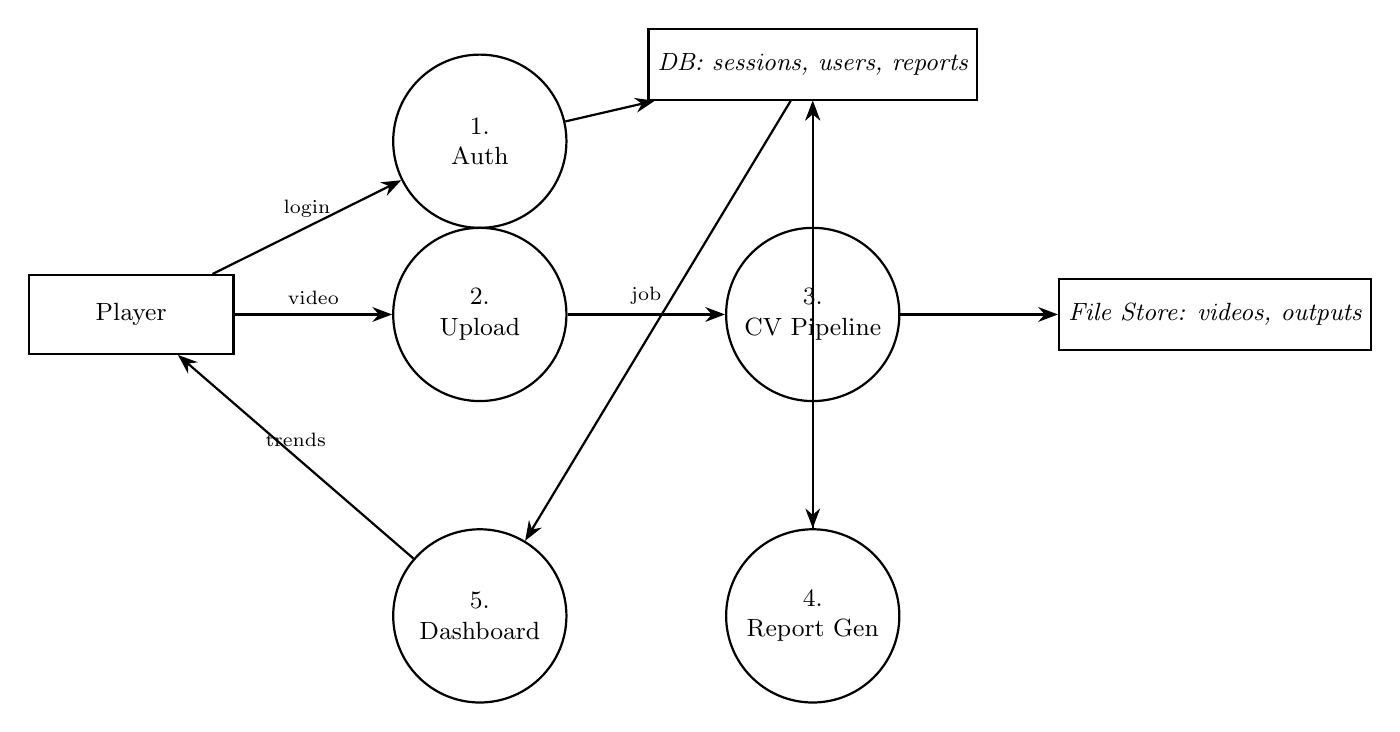
\begin{tikzpicture}[node distance=1.6cm and 2.0cm]
    \node[extproc] (user) {Player};
    \node[process, right=2.0cm of user, yshift=2.2cm] (p1) {1.\\Auth};
    \node[process, right=2.0cm of user] (p2) {2.\\Upload};
    \node[process, right=of p2] (p3) {3.\\CV Pipeline};
    \node[process, below=of p3] (p4) {4.\\Report Gen};
    \node[process, below=of p2] (p5) {5.\\Dashboard};

    \node[datastore, above=of p3] (db) {DB: sessions, users, reports};
    \node[datastore, right=of p3] (fs) {File Store: videos, outputs};

    \draw[flow] (user) -- node[above, font=\scriptsize] {login} (p1);
    \draw[flow] (user) -- node[above, font=\scriptsize] {video} (p2);
    \draw[flow] (p2) -- node[above, font=\scriptsize] {job} (p3);
    \draw[flow] (p3) -- (p4);
    \draw[flow] (p3) -- (db);
    \draw[flow] (p3) -- (fs);
    \draw[flow] (p4) -- (db);
    \draw[flow] (db) -- (p5);
    \draw[flow] (p5) -- node[above, font=\scriptsize] {trends} (user);
    \draw[flow] (p1) -- (db);
\end{tikzpicture}

\textit{Figure 2: Level 0 DFD}
\end{center}

\subsubsection*{Level 1 DFD: Process 3: CV Processing Pipeline}

\begin{center}
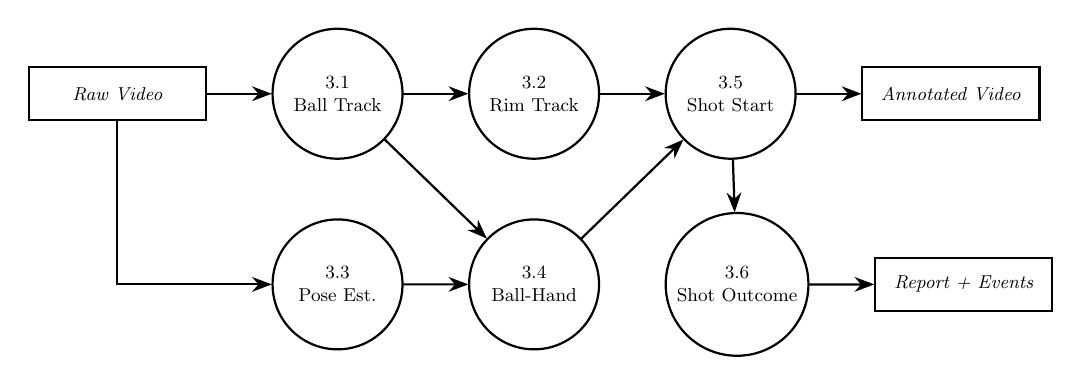
\begin{tikzpicture}[scale=0.75, transform shape, node distance=1.0cm and 1.1cm]
    \node[datastore] (in) {Raw Video};
    \node[process, right=of in] (bt) {3.1\\Ball Track};
    \node[process, right=of bt] (rt) {3.2\\Rim Track};
    \node[process, below=of bt] (pe) {3.3\\Pose Est.};
    \node[process, below=of rt] (bh) {3.4\\Ball-Hand};
    \node[process, right=of rt] (ss) {3.5\\Shot Start};
    \node[process, right=of bh] (so) {3.6\\Shot Outcome};
    \node[datastore, right=of ss] (out1) {Annotated Video};
    \node[datastore, right=of so] (out2) {Report + Events};

    \draw[flow] (in) -- (bt);
    \draw[flow] (in) |- (pe);
    \draw[flow] (bt) -- (rt);
    \draw[flow] (bt) -- (bh);
    \draw[flow] (pe) -- (bh);
    \draw[flow] (rt) -- (ss);
    \draw[flow] (bh) -- (ss);
    \draw[flow] (ss) -- (so);
    \draw[flow] (ss) -- (out1);
    \draw[flow] (so) -- (out2);
\end{tikzpicture}

\textit{Figure 3: Level 1 DFD: CV Pipeline}
\end{center}

\subsection{CRUD and Association Matrices}

\textbf{Data to Location CRUD Matrix:}

\begin{longtable}{|L{5.5cm}|c|c|}
\hline
\textbf{Entity.Attribute} & \textbf{Player (Self)} & \textbf{System (Backend)} \\ \hline
\textbf{User} & & \\ \hline
\quad .UserID & R & CRUD \\ \hline
\quad .Email & RU & CRUD \\ \hline
\quad .PasswordHash & & CRUD \\ \hline
\textbf{Session} & & \\ \hline
\quad .SessionID & R & CRUD \\ \hline
\quad .UserID & R & R \\ \hline
\quad .UploadDate & R & CRUD \\ \hline
\quad .VideoPath & & CRUD \\ \hline
\quad .Status & R & CRUD \\ \hline
\textbf{Report} & & \\ \hline
\quad .ReportID & R & CRUD \\ \hline
\quad .ShotPercentage & R & CRU \\ \hline
\quad .ConsistencyScore & R & CRU \\ \hline
\quad .FormFeedback & R & CRU \\ \hline
\textbf{ShotEvent} & & \\ \hline
\quad .FrameIndex & R & CRU \\ \hline
\quad .Outcome & R & CRU \\ \hline
\quad .ReleaseAngle & R & CRU \\ \hline
\end{longtable}

\textbf{Process to Location Association Matrix:}

\begin{tabular}{|L{6cm}|c|c|}
\hline
\textbf{Process} & \textbf{Player} & \textbf{Backend} \\ \hline
Register / Login & X & X \\ \hline
Upload Video & X & X \\ \hline
Trigger Processing & & X \\ \hline
View Results & X & X \\ \hline
View Session History & X & X \\ \hline
Delete Session & X & \\ \hline
\end{tabular}

\subsection{Use Cases}

\subsubsection*{Use Case Diagram}

\begin{center}
\begin{tikzpicture}[node distance=0.5cm and 1.4cm,
    stick/.pic={
        \draw (0,0) circle (3pt);
        \draw (0,-3pt) -- (0,-14pt);
        \draw (-6pt,-7pt) -- (6pt,-7pt);
        \draw (0,-14pt) -- (-5pt,-22pt);
        \draw (0,-14pt) -- (5pt,-22pt);
    },
    actorbox/.style={align=center, font=\small}]
    \node[actorbox] (p) {\begin{tikzpicture}\pic{stick};\end{tikzpicture}\\Player};
    \node[usecase, right=2.4cm of p, yshift=3.6cm] (uc1) {Register};
    \node[usecase, below=of uc1] (uc2) {Login};
    \node[usecase, below=of uc2] (uc3) {Upload Video};
    \node[usecase, below=of uc3] (uc4) {View Status};
    \node[usecase, below=of uc4] (uc5) {View Shot Analytics};
    \node[usecase, below=of uc5] (uc6) {View Form Analysis};
    \node[usecase, below=of uc6] (uc7) {View History};
    \node[usecase, below=of uc7] (uc8) {Delete Session};
    \node[usecase, right=3cm of uc3] (uc9) {Trigger Processing};
    \node[actorbox, right=2.4cm of uc9] (be) {\begin{tikzpicture}\pic{stick};\end{tikzpicture}\\Backend};

    \begin{scope}[on background layer]
        \node[boundary, fit=(uc1) (uc2) (uc3) (uc4) (uc5) (uc6) (uc7) (uc8) (uc9), label=above:\textbf{SwishVision System}] {};
    \end{scope}

    \foreach \u in {uc1,uc2,uc3,uc4,uc5,uc6,uc7,uc8} \draw (p) -- (\u);
    \draw (uc9) -- (be);
    \draw[->, dashed] (uc3) -- node[above, font=\scriptsize] {\textit{<<include>>}} (uc9);
    \draw[->, dashed] (uc5.east) -- ++(0.4,0) -- node[right, font=\scriptsize] {\textit{<<extend>>}} (uc7.east);
\end{tikzpicture}

\textit{Figure 4: Use Case Diagram}
\end{center}

\subsubsection*{Use Case 1: User Registration}
\begin{longtable}{|L{3.5cm}|L{11cm}|}
\hline
Use-Case Name & User Registration \\ \hline
Use-Case ID & SV-01 \\ \hline
Type & Business Requirement \\ \hline
Priority & High \\ \hline
Primary Actor & Player \\ \hline
Other Actors & System Backend \\ \hline
Description & A new user creates an account by providing name, email, and password. The system validates inputs and creates the account. \\ \hline
Precondition & The user does not already have an account with the provided email. \\ \hline
Trigger & User navigates to the registration page and submits the form. \\ \hline
Typical Course & \textbf{Actor:} provides name, email, password. \textbf{System:} validates, hashes password, stores user record, redirects to dashboard. \\ \hline
Alternate Courses & Alt 1: Email exists: error + prompt login. Alt 2: Weak password: rejected with requirements. \\ \hline
Conclusion & User account is created successfully. \\ \hline
Post Condition & User is logged in and redirected to their dashboard. \\ \hline
\end{longtable}

\subsubsection*{Use Case 2: Upload Practice Video}
\begin{longtable}{|L{3.5cm}|L{11cm}|}
\hline
Use-Case Name & Upload Practice Video \\ \hline
Use-Case ID & SV-02 \\ \hline
Type & Business Requirement \\ \hline
Priority & High \\ \hline
Primary Actor & Player \\ \hline
Other Actors & System Backend \\ \hline
Description & A logged-in user uploads a basketball practice video file. The system accepts the file, stores it, and enqueues it for processing. \\ \hline
Precondition & User is authenticated. \\ \hline
Trigger & User selects a video file and clicks Upload. \\ \hline
Typical Course & \textbf{Actor:} selects video, submits. \textbf{System:} validates format/size, stores video, creates Session (status=queued), returns job ID. \\ \hline
Alternate Courses & Alt 1: Unsupported format: rejected. Alt 2: File too large: rejected with limit message. \\ \hline
Conclusion & Video stored and queued for processing. \\ \hline
Post Condition & Session record created with status ``queued''. \\ \hline
\end{longtable}

\subsubsection*{Use Case 3: Process Video (CV Pipeline)}
\begin{longtable}{|L{3.5cm}|L{11cm}|}
\hline
Use-Case Name & Process Video \\ \hline
Use-Case ID & SV-03 \\ \hline
Type & System \\ \hline
Priority & High \\ \hline
Primary Actor & System Backend \\ \hline
Description & The backend worker picks up a queued video job and runs the CV pipeline: ball/rim tracking, pose estimation, shot detection, and report generation. \\ \hline
Precondition & A video has been uploaded and a job is queued. \\ \hline
Trigger & Background worker dequeues the job. \\ \hline
Typical Course & Runs \texttt{main\_pipeline()} on the video. Generates annotated output video, shot events, joint angle data, report text. Updates Session status to ``completed''. \\ \hline
Alternate Courses & Alt 1: Inference error: status=failed, error logged. Alt 2: No shots detected: report generated with zero shots. \\ \hline
Conclusion & Session results stored, status updated. \\ \hline
Post Condition & Session status ``completed''; Report and ShotEvent rows created. \\ \hline
\end{longtable}

\subsubsection*{Use Case 4: View Shot Analytics}
\begin{longtable}{|L{3.5cm}|L{11cm}|}
\hline
Use-Case Name & View Shot Analytics \\ \hline
Use-Case ID & SV-04 \\ \hline
Type & Business Requirement \\ \hline
Priority & High \\ \hline
Primary Actor & Player \\ \hline
Description & The user views results of a processed session: shot percentage, annotated video, per-shot outcomes, consistency score. \\ \hline
Precondition & Session status = completed. \\ \hline
Trigger & User clicks on a completed session. \\ \hline
Typical Course & \textbf{Actor:} selects session. \textbf{System:} displays shot percentage, made/missed breakdown, video player, consistency score. \\ \hline
Alternate Courses & Alt 1: Still processing: progress indicator. Alt 2: Failed: failure message with guidance. \\ \hline
Conclusion & User reviews shot data. \\ \hline
Post Condition & No state change. \\ \hline
\end{longtable}

\subsubsection*{Use Case 5: View Form Analysis}
\begin{longtable}{|L{3.5cm}|L{11cm}|}
\hline
Use-Case Name & View Form Analysis \\ \hline
Use-Case ID & SV-05 \\ \hline
Type & Business Requirement \\ \hline
Priority & High \\ \hline
Primary Actor & Player \\ \hline
Description & User views biomechanical analysis: release angle, elbow alignment feedback, consistency rating derived from joint angles. \\ \hline
Precondition & Session processed; pose data available. \\ \hline
Trigger & User navigates to Form tab of a completed session. \\ \hline
Typical Course & Displays per-shot joint angle charts, avg release angle, consistency, plain-language feedback. \\ \hline
Alternate Courses & Alt 1: Pose data unavailable: message indicating insufficient data. \\ \hline
Conclusion & User gains insight into shooting form. \\ \hline
Post Condition & None. \\ \hline
\end{longtable}

\subsubsection*{Use Case 6: View Session History}
\begin{longtable}{|L{3.5cm}|L{11cm}|}
\hline
Use-Case Name & View Session History \\ \hline
Use-Case ID & SV-06 \\ \hline
Type & Business Requirement \\ \hline
Priority & Medium \\ \hline
Primary Actor & Player \\ \hline
Description & User views a chronological list of all past sessions with summary stats and can compare metrics over time. \\ \hline
Precondition & User has at least one completed session. \\ \hline
Trigger & User navigates to History/Dashboard. \\ \hline
Typical Course & Displays sessions sorted by date with shot percentage, consistency score, trend chart. \\ \hline
Alternate Courses & Alt 1: No sessions: prompt to upload first video. \\ \hline
Conclusion & User views longitudinal progress. \\ \hline
Post Condition & None. \\ \hline
\end{longtable}

\subsubsection*{Use Case 7: Delete Session}
\begin{longtable}{|L{3.5cm}|L{11cm}|}
\hline
Use-Case Name & Delete Session \\ \hline
Use-Case ID & SV-07 \\ \hline
Type & Business Requirement \\ \hline
Priority & Low \\ \hline
Primary Actor & Player \\ \hline
Description & User permanently deletes a session and all associated data. \\ \hline
Precondition & Session belongs to authenticated user. \\ \hline
Trigger & User clicks Delete on session entry. \\ \hline
Typical Course & \textbf{Actor:} confirms deletion. \textbf{System:} removes video, report, DB records. \\ \hline
Alternate Courses & Alt 1: Session processing: deletion rejected until done. \\ \hline
Conclusion & Session and related data removed. \\ \hline
Post Condition & Session no longer in history. \\ \hline
\end{longtable}

\section{Non-Functional Requirements}

\subsection{Performance Requirements}
\begin{itemize}[leftmargin=*]
    \item Video processing should complete within a reasonable duration relative to video length, a 1-minute video within 5 minutes on a GPU server.
    \item Frontend interactions (page loads, navigation) should respond within 2 seconds under normal load.
    \item File upload should support videos up to 500\,MB without timeout.
\end{itemize}

\subsection{Safety Requirements}
\begin{itemize}[leftmargin=*]
    \item Uploaded video files stored in an isolated server directory not directly accessible via URL.
    \item Failed processing jobs caught and logged without crashing the worker.
    \item Output files verified for existence before being served to the user.
    \item Original uploaded video preserved on processing failure.
\end{itemize}

\subsection{Security Requirements}
\begin{itemize}[leftmargin=*]
    \item User passwords stored as bcrypt hashes.
    \item All user-data endpoints verify authentication and resource ownership.
    \item Upload endpoints validate MIME type and file extension.
    \item HTTPS enforced in production.
    \item Endpoints protected against common vulnerabilities.
\end{itemize}

\subsection{User Documentation}
\begin{itemize}[leftmargin=*]
    \item In-app help/onboarding for recording suitable videos and interpreting results.
    \item Developer README for environment setup and running the app.
    \item Inline tooltips for key metrics (Consistency Score, Release Angle).
\end{itemize}

\section{References}
\begin{itemize}[leftmargin=*]
    \item YOLOv8 Documentation (Ultralytics): \url{https://docs.ultralytics.com}
    \item Project Proposal: SwishVision
    \item Existing CLI codebase: \texttt{main.py} and associated tracker/drawer modules
    \item IEEE Std 830-1998: Recommended Practice for Software Requirements Specifications
\end{itemize}

\section{Appendices}

\subsection*{Appendix A: Glossary}
\begin{longtable}{|L{4cm}|L{10cm}|}
\hline
\textbf{Term} & \textbf{Definition} \\ \hline
YOLOv8 & Real-time object detection model from Ultralytics, used here for ball, rim, and pose detection. \\ \hline
Pose Estimation & CV technique that detects and tracks positions of human body joints (keypoints) in video frames. \\ \hline
Release Angle & The angle of the ball's trajectory at the point it leaves the player's hands. \\ \hline
Consistency Score & Derived metric indicating how uniform a player's shooting form is across attempts in a session. \\ \hline
Shot Event & A detected shot attempt, frame, trajectory, outcome (made/missed). \\ \hline
CV Pipeline & Chain of CV processing steps: ball tracking $\to$ rim tracking $\to$ pose estimation $\to$ shot detection $\to$ report. \\ \hline
Session & A single uploaded video and all data derived from its processing. \\ \hline
\end{longtable}

\end{document}
